\documentclass{article}
\usepackage[utf8]{inputenc}
\usepackage[english]{babel}
\usepackage[a4paper, total={7in, 9in}]{geometry}
\usepackage{graphicx}
\usepackage{float}
\usepackage{verbatim}
\usepackage{fancyvrb}
\usepackage[bottom]{footmisc}
\PassOptionsToPackage{hyphens}{url}\usepackage{hyperref}
\usepackage[style=numeric]{biblatex}
\usepackage{csquotes}
\usepackage[title]{appendix}
\usepackage{xcolor}

\addbibresource{references.bib}

\newcommand{\question}[1]{
    {\large \textbf{Q: #1}}
    \\
}

\newcommand{\titleRule}{
    \rule{\linewidth}{0.5mm} \\ [0.25cm]
}

\begin{document}

{
\center
\textsc{\Large Universidade do Minho} \\ [0.5cm]
\textsc{\Large Masters in Computer Engineering} \\ [0.5cm]
\textsc{\large Advanced Architectures} \\ [0.5cm]

{\LARGE \bfseries Matrix multiplication: Performance Analysis} \\[0.5cm]

\begin{tabular}{c c}
    José Carlos Lima Martins & Miguel Miranda Quaresma \\
    A78821 & A77049  \\
\end{tabular} \\[0.5cm]

\today \\[1cm]
}

\begin{abstract}
Performance engineering is an area of increasing importance as applications such as scientific simulations increase in complexity and require developers to be aware 
of the underlying hardware and optimization techniques available to achieve respectable performance levels. The current paper presents a walk-through of the
optimization of a dot product implementation through the application of different techniques. The impact of this techniques is measured by recording the execution
time of each kernel as well as using hardware counters to gain further insights in how each technique affects the underlying system. To aid in the optimization 
techniques a Roofline model is elaborated for the hardware platform used for testing. Several techniques are then used to improve performance, ranging from block optimization to the use of SIMD architectures such as compiler guided vectorization or GPUs (NVIDIA K20M) and many cores (KNL) to achieve peak floating point performance. 
\end{abstract}

\section{Introduction}
Parallel computing is the new paradigm for developers who wish to extract the maximum performance possible out of their applications. However, this 
paradigm doesn't dispense other optimization techniques such as vectorization or memory access locality and, in some cases, requires their use to obtain implementations that scale in modern hardware. The present work aims to implement, in an incremental way, several optimization techniques culminating in the use of two
distinct hardware approaches to high performance computing: Many Cores vs. GPUs. 

\section{Characterization of hardware platforms}
\subsection{Main laptop - hardware specifications}
The hardware specifications for the main laptop (see \ref{laptop_hardware_desc}) were obtained by 
running \verb|lscpu| and \verb|cat /proc/meminfo| in bash and by checking the manufacturer
data sheets for both the CPU(Intel 8250U) and main memory.

\subsubsection{Peak Memory Access Bandwidth - STREAM benchmark}
Off-chip (peak) memory bandwidth is one of the most determining factors in computer performance and can be measured in a number of ways, for this report the STREAM 
benchmark was used \cite{stream_bench}. To measure off-chip memory bandwidth we needed to ensure that the data used in the benchmark didn't fit in the last level of 
cache of each platform. In the case of the Intel 8285U processor, the L3 cache is non inclusive, meaning that the sum of the L2 and L3 cache($1+6=7$MiB) is used to determine the 
minimum data set size that doesn't fit in cache. As such, the following formula was used: 
\newline
$$\frac{7*1024^2}{8} = 917504 $$
\newline 
Thus the number of elements per array was set to 1048576, which yielded a total of 8MB per array. The STREAM benchmark was run 10 times and the median of the values 
was used as the peak memory bandwidth for this configuration(see \ref{stream_bench}), which was equal to:  8.899 GiB/s.

As for the Cluster node 662, the last level cache has 30MiB, thus each array was set to 4063232 elements:
$$\frac{30*1024^2}{8} = 3932160 $$

As with the main laptop, the benchmark was run 10 times and the median of the values taken as the off-chip peak memory bandwidth: 23.946 GiB/s(see \ref{stream_bench}).

One thing to note is the fact that each STREAM benchmark presents four different results, each based on the operations performed to measure memory bandwidth. Given the nature of the present work (matrix multiplication), the fourth value (\texttt{TRIAD}) was chosen, since it is the result of the following operations: \texttt{ a(i) = b(i) + q*c(i) }, which provides a more accurate representation of the operations involved in the dot product of two matrices.

\subsection{Roofline Model's}
The Roofline Model is extremely useful in identifying if and what optimizations can be applied to a given kernel \cite{roofline_model}. It does so by relating arithmetic intensity (flops/ byte) with floating point performance 
(GFlops/s) and memory performance (GiB/s) and setting a roof for the attainable performance in a given machine/configuration. 
Additionally, by defining ceilings that further limit performance according to each optimization technique (vectorization, 
memory locality, etc), it enables easy identification of the easiest optimization techniques
that result in the biggest performance gains.
For each of the hardware platforms described earlier(\ref{node662_hardware_desc} and \ref{laptop_hardware_desc}) we 
elaborated a Roofline Model using the data already presented. 
\begin{figure}[H]
    \centering
    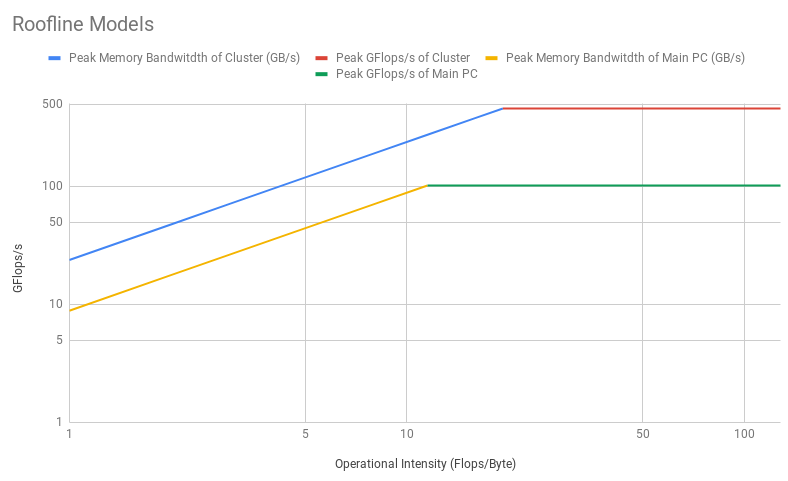
\includegraphics[width=10cm]{Pictures/roofline_merge.png}
    \caption{Merged Roofline Model w/o ceilings}
\end{figure}

One of the key takeaways from this kind of model is the maximum performance for CPU vs. Memory bound kernels. The point where both lines (peak memory bandwith
and peak floating point performance) intersect, called the ridge point, determines how hard it is to achieve maximum performance on the given configuration. With this
in mind it's possible to conclude that, as expected, the main laptop makes reaching maximum performance much easier than the cluster node. As a consequence, there
are fewer kernels that are memory bound when running in the laptop than there are when running in the cluster node, which requires an arithmetic intensity of at
least 19,24318 GFlops/byte to become CPU bound.

\subsubsection{Ceilings}
As mentioned earlier, the Roofline Model predicts the use of ceilings to limit performance according to different optimizations. This ability to predict performance 
gains based on each technique is useful when trying to decide which optimization to apply based on the possible gain it provides. Since different kernels have 
different characteristics such as the type and size of the data structures used as well as the operations performed, the following model includes the 
ceilings for the main laptop configuration for the dot product kernel and can be used as an accurate predictor of which optimizations will result in the biggest
increases in performance.
\begin{figure}[H]
    \centering
    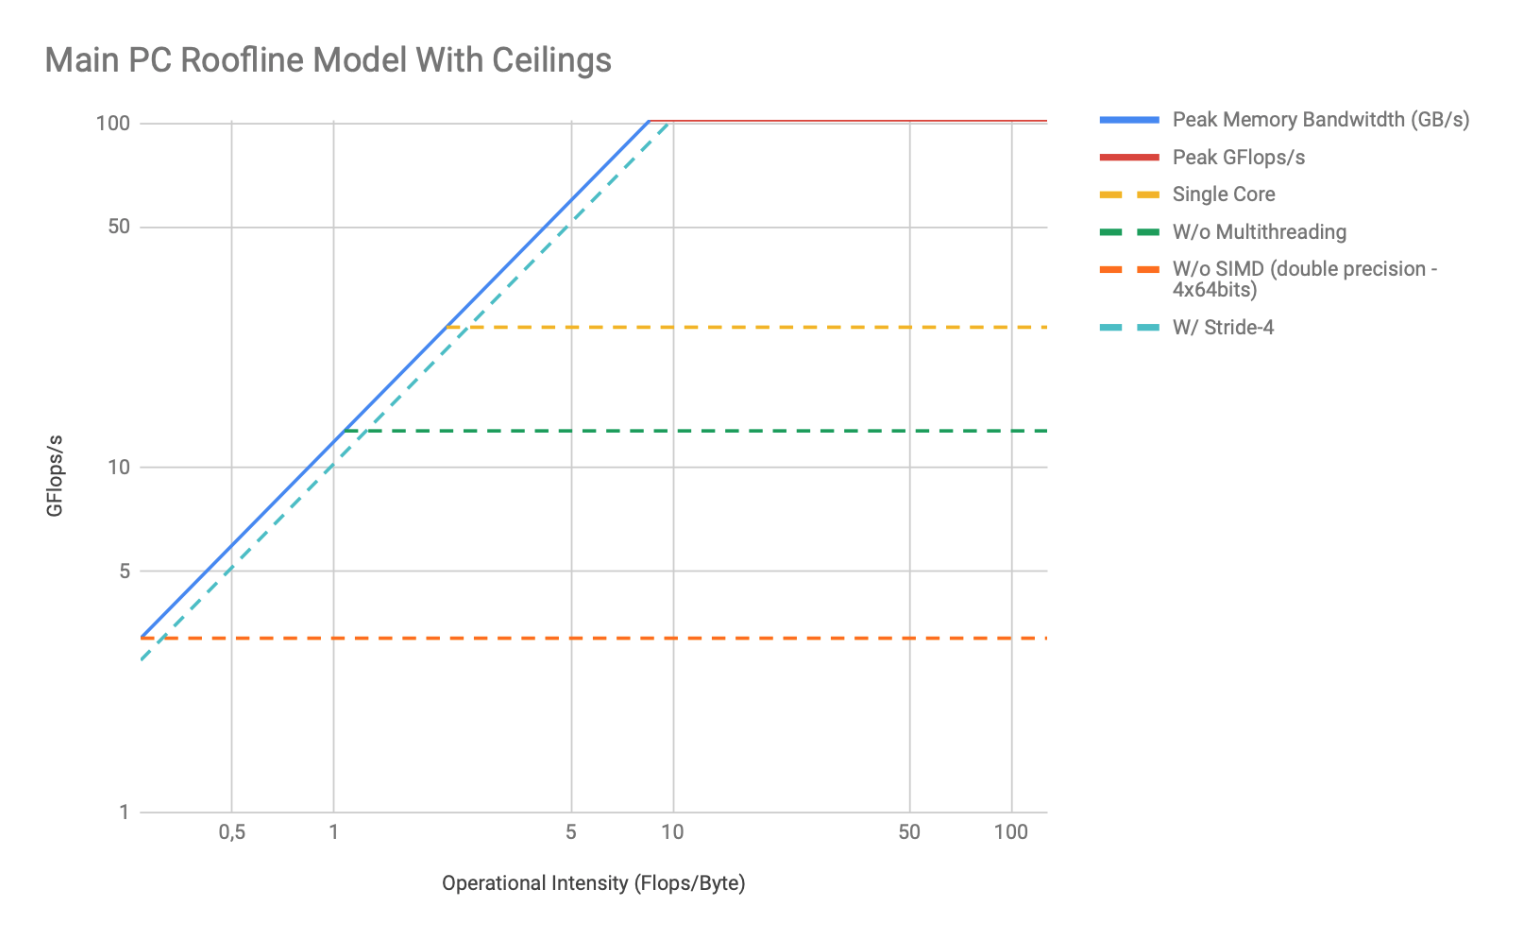
\includegraphics[width=10cm]{Pictures/roofline_mainpc_ceilings.png}
\caption{Main laptop roofline Model w/ ceilings}
\end{figure}

To determine the impact of each optimization on the performance ceiling it is often useful to either consult the manufacturer manual for optimization techniques or 
perform benchmarks that allow a comparison between optimized and non-optimized versions of a kernel. In this case, the strided access impact on memory bandwidth was 
obtained by modifying the STREAM benchmark to support strided access, in this case stride-4.
The multi-core and multithreaded performance impacts were determined by taking the number of cores (and threads) and dividing the achievable performance by these,
assuming a linear improvement in function of the number of cores(threads) used, since the Intel i5-8250U has 4 cores, this sets the ceiling at: $$\frac{102.4}{4} = 25.6 GFLOP/s$$
Using multi-threading allows for two threads to run concurrently in each core, meaning the absence of this technique further limits attainable performance to half the possible value: $$\frac{25.6}{2} = 12.8 GFLOP/s$$
As for the impact of vectorization, the width of the vector units was taken into account, in this case it supports 4 doubles, meaning the expected impact is, at most,
4 times the achievable performance, setting the ceiling at: $$\frac{12.8}{4} = 3.2 GFLOP/s$$

\section{Analysis of different matrix dot product implementations}
\subsection{PAPI - Performance API}
The Performance API(PAPI) is a useful tool for identifying bottlenecks and analyzing program execution. Due to the considerable amount of 
(hardware) counters made available by the API, it's paramount to identify the relevant ones on a use-case basis.

The available counters are dependent on the (hardware) platform, therefore we must first describe the hardware used for this study. This description is available in appendix in the section \ref{node662_hardware_desc}.

To list the available counters we must first load the PAPI module(version 5.5.0) by issuing the command \texttt{module load papi/5.5.0} and, 
by running \texttt{papi\_avail}, we obtain a comprehensive list of the commands provided by PAPI and an indicator on whether the platform supports them or not.

From this list we selected the following counters:
\begin{Verbatim}[fontsize=\footnotesize]
PAPI_L1_DCM - Level 1 data cache misses
PAPI_L2_DCM - Level 2 data cache misses
PAPI_L2_TCM - Level 2 cache misses
PAPI_L3_TCM - Level 3 cache misses
PAPI_L1_LDM - Level 1 load misses
PAPI_L1_STM - Level 1 store misses
PAPI_L2_STM - Level 2 store misses
PAPI_TOT_INS - Instructions completed
PAPI_FP_INS - Floating point instructions
PAPI_LD_INS - Load instructions
PAPI_SR_INS - Store instructions
PAPI_L2_DCH - Level 2 data cache hits
PAPI_L2_DCA - Level 2 data cache accesses
PAPI_L3_DCA - Level 3 data cache accesses
PAPI_L3_TCA - Level 3 total cache accesses
PAPI_L3_DCW - Level 3 data cache writes
\end{Verbatim}

The counters referring to cache data, such as misses and accesses, loads and stores, 
allow us to determine how much the application is taking advantage of the memory 
hierarchy and whether it's possible to increase memory locality to reduce the 
amount of misses or, in case it isn't, whether it's advantageous to use multiple threads
to hide memory latency.

The counter for the number of instructions completed is necessary to calculate the 
execution time of an application. 
The floating point instruction counter will be useful to calculate floating point performance and,
when used in conjunction with memory access counters, can be used to determine the 
arithmetic intensity(Flops/byte) of the dot product kernel.


\subsection{Data Structures for a r662 node}
To implement the dot product algorithm we need three NxN matrices of floats which sets the required size to $3*N*N*4\ bytes$, (where 4 is the size of a float, in 
bytes). Solving this equation for each cache level size gives us the amount of elements that completely fill each one. The cache sizes for the r662 node can be found in the section \ref{node662_hardware_desc}:
\begin{itemize}
    \item Fits in L1 cache: $N = 52 $ 
    \item Fits in L2 cache: $N = 128$ 
    \item Fits in L3 cache: $N = 1024$
    \item Only fits in main memory: (at least 1619) $N = 2048$
\end{itemize}
The equations for each cache level can be checked in the Appendix \ref{general_mem_formula}. One thing to note is the choice of powers of 2 for the number of elements
per row/column which makes it easier to implement certain optimization techniques such as vectorization by allowing aligned accesses. 

\subsection{Memory metrics}
Memory bandwidth is one of the biggest bottlenecks in modern computing with CPU speeds greatly surpassing those of main memory as such, without the use of memory latency hiding techniques, the CPU would spend most of the time waiting for data to be fetched from memory.  
Consequently it's of paramount importance to find ways to limit the amount of times main memory is accessed favoring the smaller but faster memories that are closer
to the CPU and thus present reduced latency in comparison to bigger memories. This can be achieved through the use of several techniques that affect different metrics 
which we'll identify in the current section.

\subsubsection{Theoretical methods}
The best execution time for each dot product corresponds to the smallest matrix size \textbf{i.e.} N=52, when the matrix fits completely in L1 cache. As such the
number of RAM accesses per instruction as well as the amount of bytes transferred to/from RAM can be estimated based on this assumptions, as a function of the matrix 
size:
\begin{itemize}
    \item Number of RAM accesses per instruction $ \approx 1/32$[Eq: \ref{acessesEq}]
    \item Number of bytes transferred to RAM $\approx N*N*N*4 \Leftrightarrow 562432 (N=52)$ [Eq: \ref{bytesToRAM}]
    \item Number of bytes transferred from RAM $\approx N*N*N*4*3 \Leftrightarrow 1687296 (N=52)$ [Eq: \ref{bytesFromRAM}]
\end{itemize}

\subsubsection{With PAPI counters}

Being approximations it's useful to confirm the values with real data which can be obtained via PAPI. Using that
data we can develop, for each counter, an expression which calculates the value:
\begin{itemize}
    \item Number of RAM accesses per instruction: \texttt{PAPI\_TOT\_INS, PAPI\_L3\_TCM} [Eq: \ref{acessesEq_papi}]
    \item Number of bytes transferred to RAM: \texttt{PAPI\_SR\_INS}[Eq: \ref{bytesToRAM_papi}]
    \item Number of bytes transferred from RAM: \texttt{PAPI\_LD\_INS} [Eq: \ref{bytesFromRAM_papi}]
\end{itemize}

\subsubsection{Miss rate on reads - Kernel j-k-i}
As previously said, one of the major bottlenecks in computer performance is main memory. When a \texttt{load} instruction is executed,
neglecting operand pre-fetch techniques, the address being loaded is searched for in the higher levels of memory hierarchy and, when it
isn't found it occurs what is known as a miss, a read miss. This miss causes the CPU to search in the next level of the memory hierarchy
which is slower and incurs the CPU in wasted memory cycles waiting for the operand to be loaded. As such read miss rate is an extremely 
important metric in examining the behaviour of an application and can be calculated by resorting to PAPI counters for each cache 
level(see Appendix \ref{miss_rate}).

\subsection{Kernel Plotting in Roofline model}
The number of floating point operations performed in any given kernel is given by the following expression: $ (1 + 1) * N^3$ 
where $(1+1)$ corresponds to the multiplication and addition operations performed in each inner loop iteration 
and $N^3$ to the total number of iterations of that loop.
Thus, for each data set size, the number of floating point operations performed is:
\begin{itemize}
    \item \textbf{N=52} : 281216 Flops 
    \item \textbf{N=128} : 4194304 Flops
    \item \textbf{N=1024} : 2147483648 Flops
    \item \textbf{N=2048} : 17179869184 Flops
\end{itemize}
Using the Roofline models previously elaborated we're now able to plot the achieved performance (see \ref{plot_achieved_roofline}) which, as expected, is well below the theoretical limit for the cluster node 662. This is caused by the lack
of any optimizations such as improved memory locality, vectorization or multiprocessing.

\subsection{Performance limiting factors - Memory vs CPU}
Analyzing the results of the achieved performance (see Appendix \ref{plot_achieved_roofline}) it's obvious that one of the limiting factors to performance is memory
bandwidth, which can be improved by taking advantage of the caches closer to the CPU.

Another key takeaway from the values obtained (see Appendix \ref{non_optimized}) is that memory access patterns are of paramount importance and ought to be considered 
for applications concerned with performance. In this case, interchanging the loop order (\textbf{i-j-k}, \textbf{i-k-j}, \textbf{j-k-i}) greatly impacts performance based on whether matrices
are accessed in a row-major or column-major mode. The results show that the \textbf{i-k-j} obtained the best results by 
exhibiting better spacial locality than \textbf{j-k-i} and \textbf{i-j-k} and better temporal locality, therefore taking advantage of cache and memory hierarchy.
Furthermore, the \textbf{j-k-i} version of the dot product clearly benefits from matrix transposition which, by rearranging the way each matrix is stored in memory, allows for
better spacial and temporal locality.

\subsection{Optimization Techniques}
\subsubsection{Block dot product}
The block optimization in dot product increases the spacial locality of columns and rows, decreasing the number of  replacements of 
cache lines and improving the execution time of the dot product. Without blocks, if the rows are large enough to not fit in a single cache 
line, there will be a high number of collisions when loading values and, thus repeated loads and replacements of cache lines. The use of blocks 
prevents this by limiting the size of each block so that each row fits in a single cache line, reducing the number of collisions making the 
amount of misses come closer to that the amount of cold misses. 

\subsubsection{Vectorization}
Vectorization is another technique whose main objective is to hide memory latency and improve parallelism at the data level. It works by loading a vector from memory 
and operating on the elements of that vector simultaneously. Modern compilers are already able to identify vectorizable portions of code which normally only involve
loops that perform arithmetic calculations on vector elements with no dependencies across iterations. 
Thus, the current implementation of the dot product with block optimization, represents an almost perfect candidate for being vectorized by the compiler. One of the 
issues that needs to be solved prior is the alignment of vector memory addresses which should be 16 byte aligned. This can be achieved by declaring the pointers with the \texttt{aligned} modifier, as such:
\begin{Verbatim}[fontsize=\small]
float __attribute__((aligned(32))) **a = ...
float __attribute__((aligned(32))) **b = ...
float __attribute__((aligned(32))) **c = ...
\end{Verbatim}
Another obstacle to auto-vectorization by the compiler is pointer aliasing, in this case:
\begin{Verbatim}[fontsize=\small]
void dotProductBlockOptimized(float **c, 
                              float **a, 
                              float **b, 
                              int n){
    ...
    c[i][j] += a[i][k] * b[k][j]; 
\end{Verbatim}
the compiler won't vectorize the code because pointers \texttt{a,b} and \texttt{c} may point to the same memory location. To prevent this from happening the 
\texttt{\_\_restrict\_\_} keyword indicates that the pointer to which it is applied is the only alias to that memory location:
\begin{Verbatim}[fontsize=\small]
void dotProductBlockOptimized(float ** __restrict__ c, 
                              float ** __restrict__ a, 
                              float ** __restrict__ b, 
                              int n)
\end{Verbatim}
Besides increasing data level parallelism and hiding memory latency, vectorization also reduces the amount instructions needed to execute a given kernel since
each vector instruction performs the equivalent of 8 scalar instructions. 
Observing the results of applying this technique it's visible that the obtained speed-up ($\approx 5.66$x)~(see \ref{fig:speedUpVec}) is lower than the expected speed-up ($\approx 8$x). 
This is because loading a vector from memory demands more bandwidth than loading a single value, putting more load on memory (bandwidth) and lowering achieved 
performance. 
\subsubsection{Multicore processing}
Multicore processing is another form of parallelism that allows for the work load to be distributed among cores, reducing the time it takes to executed a parallel 
region of code significantly. The use of APIs such as OpenMP make adapting codes with high parallel potential trivial, though care has to be taken for shared 
variables and memory dependencies.
Applying this technique to the dot product kernel involved adding a \texttt{pragma} directive before the inner-most loop to parallelize that region. For the tests 24 threads were used which would result, theoretically, in a 24x speed-up however the results show a larger speed-up due to the fact that this optimization technique was combined with vectorization, yielding a 37.58x speed-up~(see \ref{fig:exeTimeMulti}). Yet again, this is far from
the expected speed-up when we take into account vectorization, which would be $8*24=192$x which can be justified by the fact that we now have 24 threads sharing the last level cache as well as the memory bandwidth, hence why the speed-up is lower than expected.
\subsubsection{Kepler GPU}
The amount of floating-point units in GPUs and the easy implementation made possible by platforms like CUDA have made this devices one of the tools for high 
performance computing. The use of high amounts of floating point units allows memory latency to be hidden by switching between thread groups, known as warps, when 
data isn't yet available. GPUs follow "Same Instruction Multiple Threads" model which means that the threads in a warp will execute the same instruction on 
different operands.
On the other hand, many of the control mechanisms involved in this process are implemented in hardware making it transparent to the developer.
The implementation of the dot product algorithm on a GPU using CUDA consisted on adapting the current implementation to the CUDA model where each (CUDA) thread processes only one element of the data set: 
\begin{Verbatim}[fontsize=\small]
*(dev_result+blockIdx.x*N+threadIdx.x)=0;

for(unsigned i=0; i < N; i++)
	*(dev_result+blockIdx.x*N+threadIdx.x) += *(dev_m1+blockIdx.x*N+i) * *(dev_m2+i*N+threadIdx.x); 
\end{Verbatim}
As expected there was a visible increase in performance(see \ref{kepler_k20m} and \ref{non_optimized}) with most of execution time of the 
GPU implementation being attributed to the communication between the host(CPU) and the device(GPU) which accounted for almost 99\% of the total execution time.

\subsubsection{KNL - Coprocessor}
Coprocessors such as the KNL architecture are an alternative to GPUs when it comes to executing highly parallel kernels. Known as manycore processors this devices are 
similar to GPUs in that they're focused on being efficient for executing highly parallel code, with manycores requiring that this parallelism be explicit. A distinct 
advantage of the KNL coprocessor over a CUDA GPU is the fact that applications developed for running on multicore processors are meant to be portable/compatible with 
manycores which isn't the case for GPUs.
Another advantage of manycores over GPUs is the ability to run sequential code in a more efficient manner than the latter, making them more suited for irregular workloads \cite{xmt_gpu}. The results obtained with the KNL Coprocessor present a considerable speed-up in comparison to the base version due to the exploitation of the high parallelism available in the dot product but fall short when compared to the Kepler GPU (see \ref{fig:speedUpAcc}).

\section{Conclusion}
The use of matrices in scientific applications is frequent, as such the results obtained not only offer valuable insights on how to develop efficient code while also 
remaining useful for other application types that use similar data structures. Furthermore, the results show that the use of kernels that access memory in an optimal way, such as the i-k-j kernel, present the best performance. Additionally, although the communication between the GPU and the CPU is a major bottleneck for 
performance, the use of a GPU still presented better results than the use of a manycore when executing the dot product kernel (see \ref{fig:generalSpeedUp}). 

\printbibliography

\newpage 
\begin{appendices}

\section{Full characterization of the hardware platform}

\subsection{SeARCH Cluster node 662}
\label{node662_hardware_desc}
\begin{itemize}
    \item (Dual) CPU:
        \begin{itemize}
            \item Manufacturer: Intel
            \item Model: Xeon E5-2695 v2 
            \item Number of cores: 12
            \item Peak FP performance: 460.8 GFlops/s ~\cite{flops, flopsCalc}
        \end{itemize}
    \item Main Memory:
        \begin{itemize}
            \item Size: 64 GB
        \end{itemize}
    \item Memory Hierarchy:
        \begin{itemize}
            \item Cache sizes and associativity:
                \begin{itemize}
                    \item L1d (per core): 32 KiB, 8-way
                    \item L1i (per core): 32 KiB, 8-way
                    \item L2 (per core): 256 KiB, 8-way
                    \item L3 (per package): 30 MiB, 20-way
                \end{itemize}
            \item Memory access bandwidth: 23.94614 GB/s
        \end{itemize}
    \item Extras:
        \begin{itemize}
            \item GPU: 2x Nvidia K20m \cite{GPU,K20,GK110}
            \begin{itemize}
                \item Cuda Cores: 2496 (each one with FP and Integer unit)
                \item SMX: 13
                \begin{itemize}
                    \item Threads / Warp: 32
                    \item Max Threads / Thread Block: 1024
                    \item Max Warps / Multiprocessor: 64
                    \item Max Threads / Multiprocessor: 2048
                    \item Max Thread Blocks / Multiprocessor: 16
                \end{itemize}
                \item Cuda Cores per SMX: 192
                \item Double Precision Units: 64 (divided in 4 ``lanes'' of 16 units)
                \item Local Memory: 65536 x 32-bit registers
                \item Shared Memory: 64 KiB divided between shared memory and L1 cache, configurable; 48 KiB Read-Only Data Cache
                \item Global Memory: 5GB (GDDR5)
                \item GPU Clock: 706 MHz
                \item Memory Clock: 2.6 GHz
            \end{itemize}
            \item Coprocessor: Intel(R) Xeon Phi(TM) CPU 7210 \cite{KNL}
            \begin{itemize}
                \item Frequency: 1.3 GHz
                \item Cores: 64
                \item Threads: $64*4 = 256$
                \item Cache:
                \begin{itemize}
                    \item L1 Data (per core): 32 KiB
                    \item L1 Instructions (per core): 32 KiB
                    \item L2: $32 * 1024 KB = 32MB$
                \end{itemize}
                \item On Package Memory: 16 GB with 8 channels
            \end{itemize}
        \end{itemize}
\end{itemize}

\subsection{Main laptop - hardware specifications}
\label{laptop_hardware_desc}
\begin{itemize}
    \item Manufacturer: Asus
    \item Model: VivoBook S14 S410UN
    \item CPU:
        \begin{itemize}
            \item Manufacturer: Intel
            \item Model: i5-8250U 1.60GHz
            \item Reference: 124967
            \item Number of cores: 4 cores, 8 threads (Hyper-Threading)
            \item Peak FP performance: 102.4 GFlops/s ~\cite{flops,flopsCalc}
        \end{itemize}
    \item Main Memory:
        \begin{itemize}
            \item Memory Frequency: 2667 Mhz (Tcc = 0.4 ns)
            \item CL (Column access strobe Latency): 15
            \item Latency: 6 ns (= 15 * 0.4 ns)
            \item Size: 8 GB
        \end{itemize}
    \item Memory Hierarchy:
        \begin{itemize}
            \item Cache sizes and associativity:
                \begin{itemize}
                    \item L1d (per core): 32 KiB, 8-way
                    \item L1i (per core): 32 KiB, 8-way
                    \item L2 (per core): 256 KiB, 4-way
                    \item L3 (per package): 6144 KiB, 12-way
                \end{itemize}
            \item Memory access bandwidth: 9112.2 MB/s 
        \end{itemize}
\end{itemize}
\subsection{STREAM benchmark}
\label{stream_bench}
\begin{figure}[H]
    \centering
    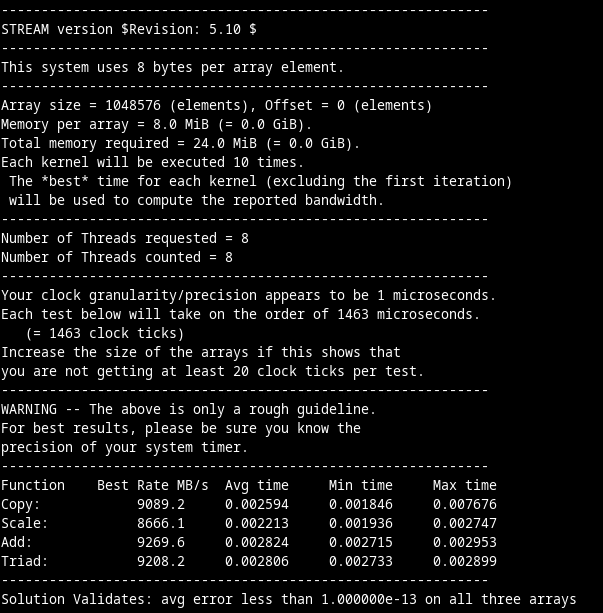
\includegraphics[scale=0.3]{Pictures/StreamBench_AsusS410UN.png}
    \caption{STREAM benchmark output for the main laptop}
\end{figure}

\begin{figure}[H]
    \centering
    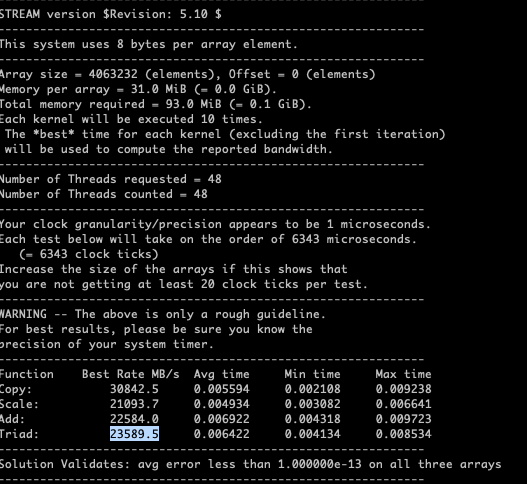
\includegraphics[scale=0.35]{Pictures/StreamBench_Node662.png}
    \caption{STREAM benchmark output for 662 Cluster node}
\end{figure}

\section{Available PAPI Counters - Node 662}
\begin{Verbatim}[fontsize=\footnotesize]
    Name     Deriv Description (Note)
PAPI_L1_DCM   No   Level 1 data cache misses
PAPI_L1_ICM   No   Level 1 instruction cache misses
PAPI_L2_DCM   Yes  Level 2 data cache misses
PAPI_L2_ICM   No   Level 2 instruction cache misses
PAPI_L1_TCM   Yes  Level 1 cache misses
PAPI_L2_TCM   No   Level 2 cache misses
PAPI_L3_TCM   No   Level 3 cache misses
PAPI_TLB_DM   Yes  Data translation lookaside buffer misses
PAPI_TLB_IM   No   Instruction translation lookaside buffer misses
PAPI_L1_LDM   No   Level 1 load misses
PAPI_L1_STM   No   Level 1 store misses
PAPI_L2_STM   No   Level 2 store misses
PAPI_STL_ICY  No   Cycles with no instruction issue
PAPI_BR_UCN   Yes  Unconditional branch instructions
PAPI_BR_CN    No   Conditional branch instructions
PAPI_BR_TKN   Yes  Conditional branch instructions taken
PAPI_BR_NTK   No   Conditional branch instructions not taken
PAPI_BR_MSP   No   Conditional branch instructions mispredicted
PAPI_BR_PRC   Yes  Conditional branch instructions correctly predicted
PAPI_TOT_INS  No   Instructions completed
PAPI_FP_INS   Yes  Floating point instructions
PAPI_LD_INS   No   Load instructions
PAPI_SR_INS   No   Store instructions
PAPI_BR_INS   No   Branch instructions
PAPI_TOT_CYC  No   Total cycles
PAPI_L2_DCH   Yes  Level 2 data cache hits
PAPI_L2_DCA   No   Level 2 data cache accesses
PAPI_L3_DCA   Yes  Level 3 data cache accesses
PAPI_L2_DCR   No   Level 2 data cache reads
PAPI_L3_DCR   No   Level 3 data cache reads
PAPI_L2_DCW   No   Level 2 data cache writes
PAPI_L3_DCW   No   Level 3 data cache writes
PAPI_L2_ICH   No   Level 2 instruction cache hits
PAPI_L2_ICA   No   Level 2 instruction cache accesses
PAPI_L3_ICA   No   Level 3 instruction cache accesses
PAPI_L2_ICR   No   Level 2 instruction cache reads
PAPI_L3_ICR   No   Level 3 instruction cache reads
PAPI_L2_TCA   Yes  Level 2 total cache accesses
PAPI_L3_TCA   No   Level 3 total cache accesses
PAPI_L2_TCR   Yes  Level 2 total cache reads
PAPI_L3_TCR   Yes  Level 3 total cache reads
PAPI_L2_TCW   No   Level 2 total cache writes
PAPI_L3_TCW   No   Level 3 total cache writes
PAPI_FDV_INS  No   Floating point divide instructions
PAPI_FP_OPS   Yes  Floating point operations
PAPI_SP_OPS   Yes  Floating point operations; optimized to count scaled single precision vector operations
PAPI_DP_OPS   Yes  Floating point operations; optimized to count scaled double precision vector operations
PAPI_VEC_SP   Yes  Single precision vector/SIMD instructions
PAPI_VEC_DP   Yes  Double precision vector/SIMD instructions
PAPI_REF_CYC  No   Reference clock cycles 
\end{Verbatim}

\section{Peak floating point performance formulas}
\subsection{Cluster 662 Node}
\begin{equation}
2.4 (frequency) * 12 (cores) * 8 (DFlops\_per\_cycle) * 2 (cpu's\_per\_node)) = 460.8 GFlops/s \\
\end{equation}

\subsection{Main laptop}
\label{main_laptop_flop}
\begin{equation}
1.6 (frequency) * 4 (cores) * 16 (DFlops\_per\_cycle) * 1 (cpu's\_per\_node)) = 102.4 GFlops/s \\
\end{equation}

\section{Matrix size formulas}
\subsection{General formula}
\label{general_mem_formula}
\begin{equation}
no_{matrices} * matrix\_order * float\_size = memory\_size 
\end{equation}

\subsection{Matrix fitting in L1 cache}
\begin{equation}
3*N*N*4 = 32 * 1024 \Leftrightarrow N \approx 52 
\end{equation}

\subsection{Matrix fitting in L2 cache}
\begin{equation}
3*N*N*4 = 256*1024 \Leftrightarrow N \approx 147 
\end{equation}

\subsection{Matrix fitting in L3 cache}
\begin{equation}
3*N*N*4 = 30*1024^2 \Leftrightarrow N \approx 1619
\end{equation}

\subsection{Matrix fitting in L3 cache for Multicore}
\begin{equation}
3*N*N*4 = \frac{2*30*1024^2}{24} \Leftrightarrow N \approx 467
\end{equation}

\section{Non optimized dot product measurements}
\label{non_optimized}
\begin{tabular}{|c|c|c|c|c|}
\hline
              & {i-j-k}                     & i-k-j                        & j-k-i                    & j-k-i (transposed)                \\
\hline
Matrix Order  & K-Best(K=3)(us)             & K-Best(K=3)(us)              & K-Best(K=3)(us)          & K-Best(K=3)(us)                   \\ 
\hline \hline
 52           & 199,00$\pm$9,95            & 174.00$\pm$8.70             & 239.67$\pm$11.98        & 207.67$\pm$10.38                 \\
\hline
 128          & 2823,33$\pm$141,17         & 2616$\pm$130.8              & 3296.33$\pm$164.82      & 2956.33$\pm$147.82               \\
\hline
 1024         & 8297943,33$\pm$414897,17   & 1346980.333$\pm$67349.02    & 10388926$\pm$519446.30  & 10686387.67$\pm$534319.38        \\
\hline
 2048         & 49543536,67$\pm$2477176,83 & 10789776.33$\pm$539488.82   & 72615491,67$\pm$3630774,58 & 34268445,67$\pm$1713422,28    \\ 
\hline
\end{tabular}
\newline

\footnotesize{\textbf{n.b.}results are shown with 5\% tolerance}

\section{RAM Access - Theoretical formulas}
\subsection{Bytes transferred to RAM}
\begin{equation}
N*N*N*4\label{bytesToRAM}
\end{equation}
with N=matrix order and 4=float size in bytes

\subsection{Bytes transferred from RAM}
\begin{equation}
N*N*N*4*3\label{bytesFromRAM}
\end{equation}
with N=matrix order, 4=float size in bytes and 3=no. of matrices

\subsection{RAM Accesses per Instruction}
\begin{equation}
\frac{\frac{3*N^3}{16}}{6*N^3} = \frac{1}{32}\label{acessesEq}
\end{equation}

\section{RAM Access - PAPI formulas}
\subsection{Bytes transferred to RAM}
\begin{equation}
PAPI\_SR\_INS*4\label{bytesToRAM_papi}
\end{equation}
with 4=float size in bytes

\subsection{Bytes transferred from RAM}
\begin{equation}
PAPI\_LD\_INS*4\label{bytesFromRAM_papi}
\end{equation}
with 4=float size in bytes

\subsection{RAM Accesses per Instruction}
\begin{equation}
\frac{PAPI\_L3\_TCM}{PAPI\_TOT\_INS} \label{acessesEq_papi}
\end{equation}

\section{Achieved Performance Plot in Roofline Models}
\label{plot_achieved_roofline}

\begin{figure}[H]
    \centering
    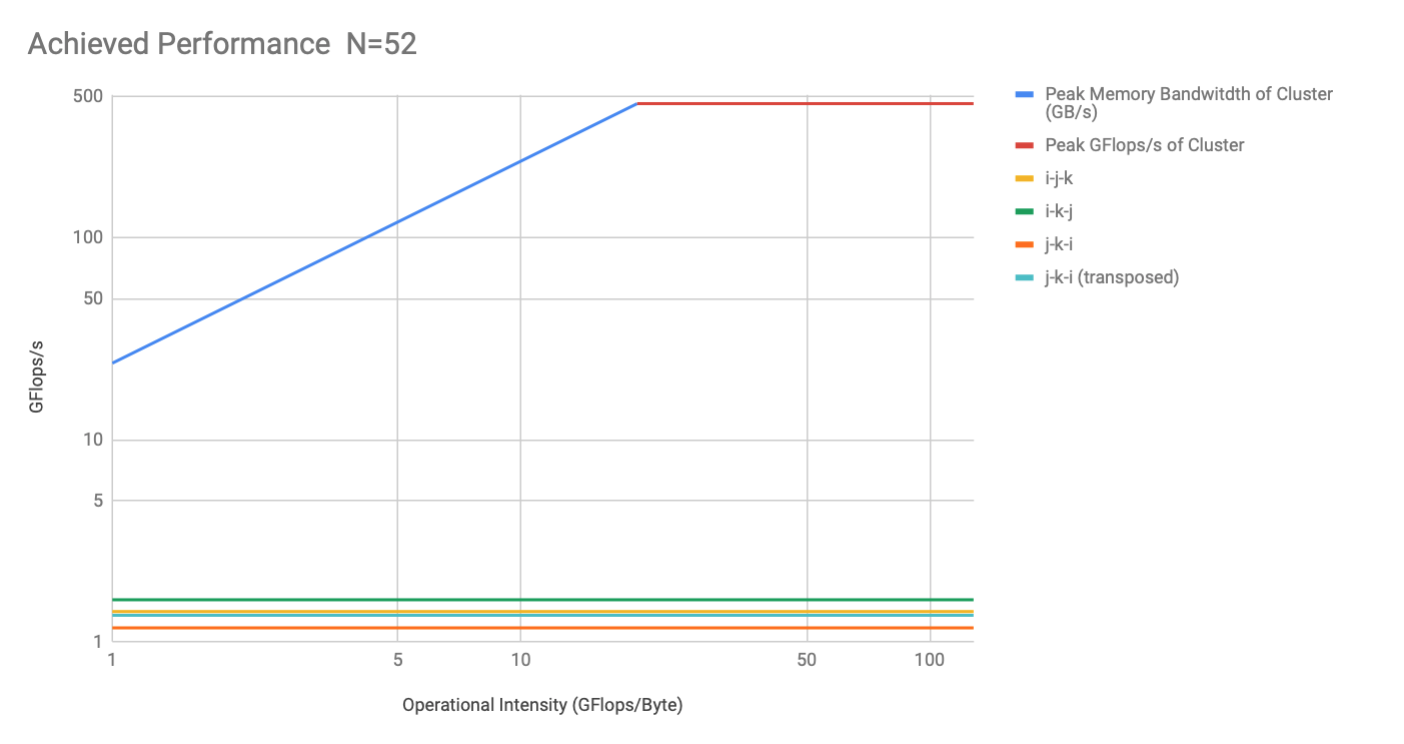
\includegraphics[width=15cm]{Pictures/roofline_ap_52.png}
    \caption{Achieved Performance for N=52}
    \label{fig:roofline_ap_52}
\end{figure}

\begin{figure}[H]
    \centering
    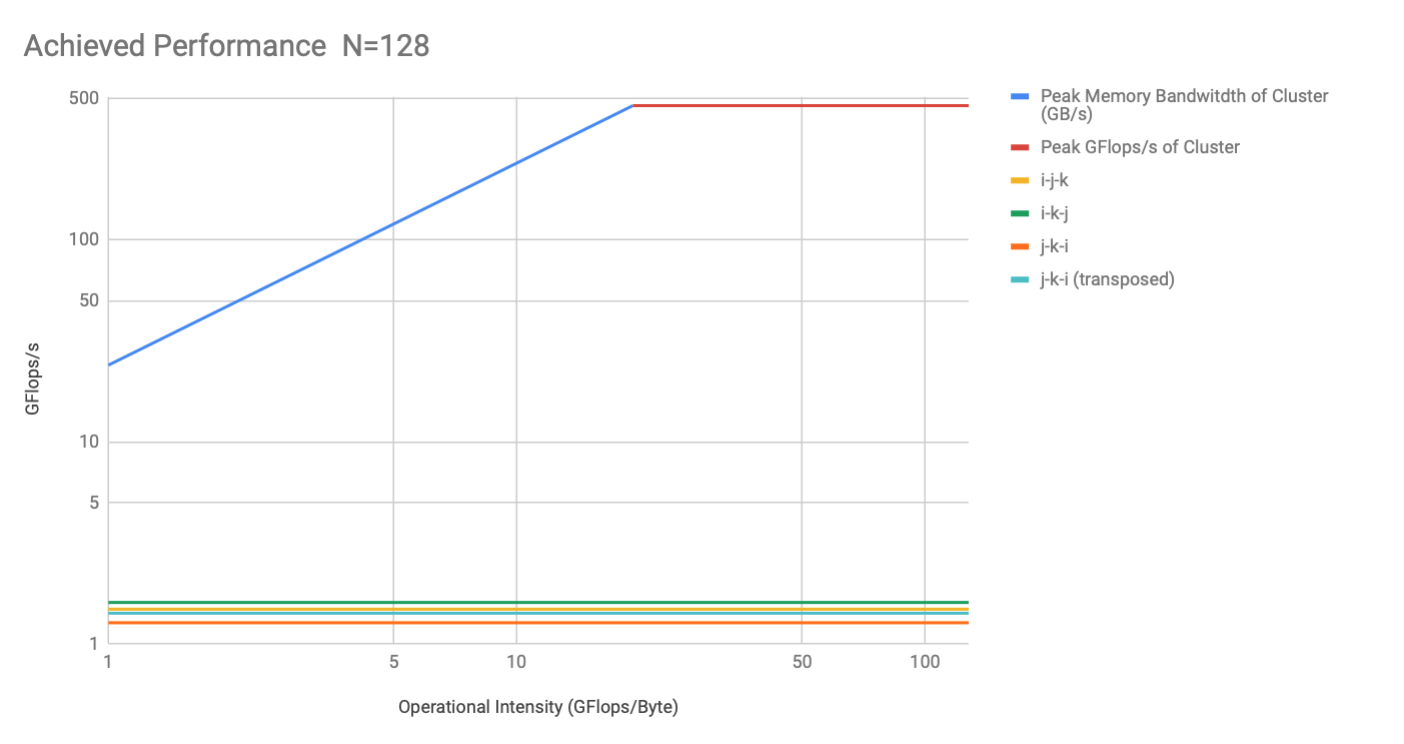
\includegraphics[width=15cm]{Pictures/roofline_ap_128.png}
    \caption{Achieved Performance for N=128}
    \label{fig:roofline_ap_128}
\end{figure}

\begin{figure}[H]
    \centering
    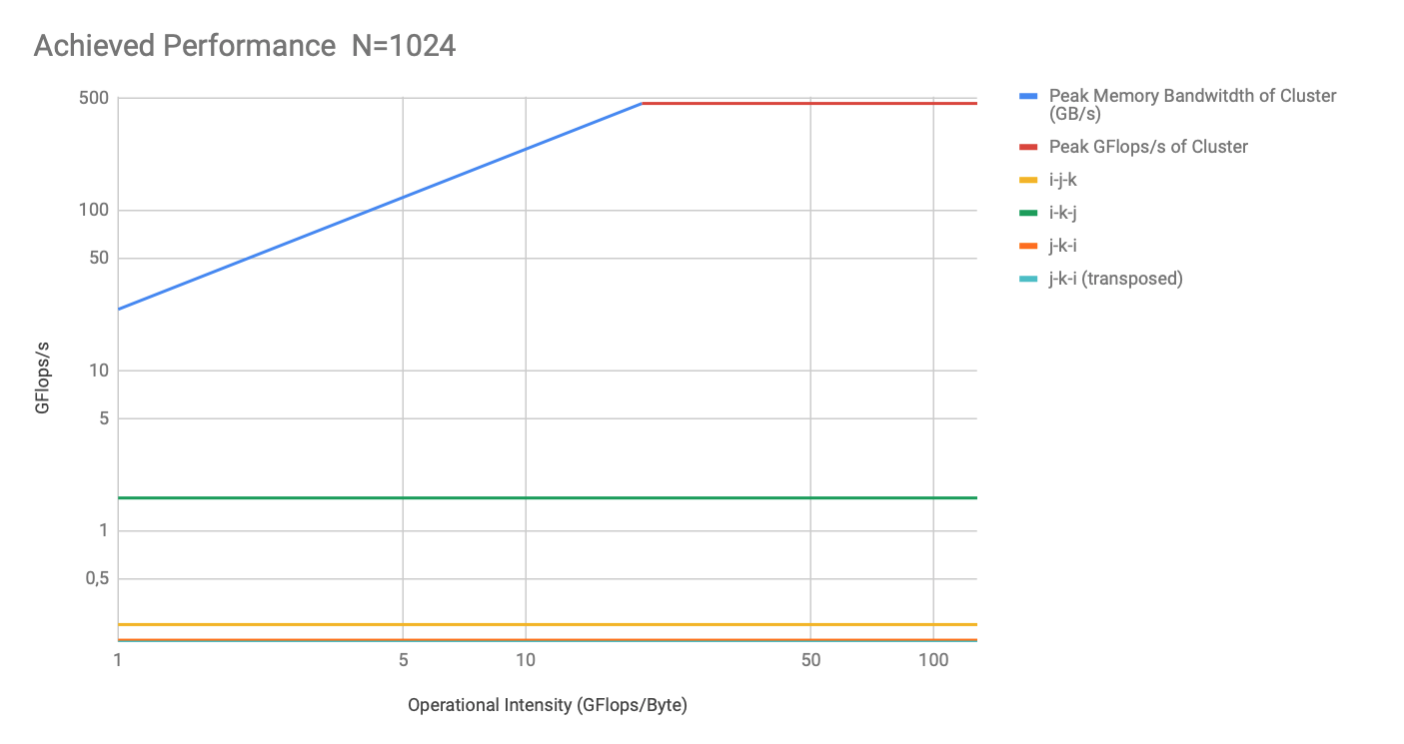
\includegraphics[width=15cm]{Pictures/roofline_ap_1024.png}
    \caption{Achieved Performance for N=1024}
    \label{fig:roofline_ap_1024}
\end{figure}

\begin{figure}[H]
    \centering
    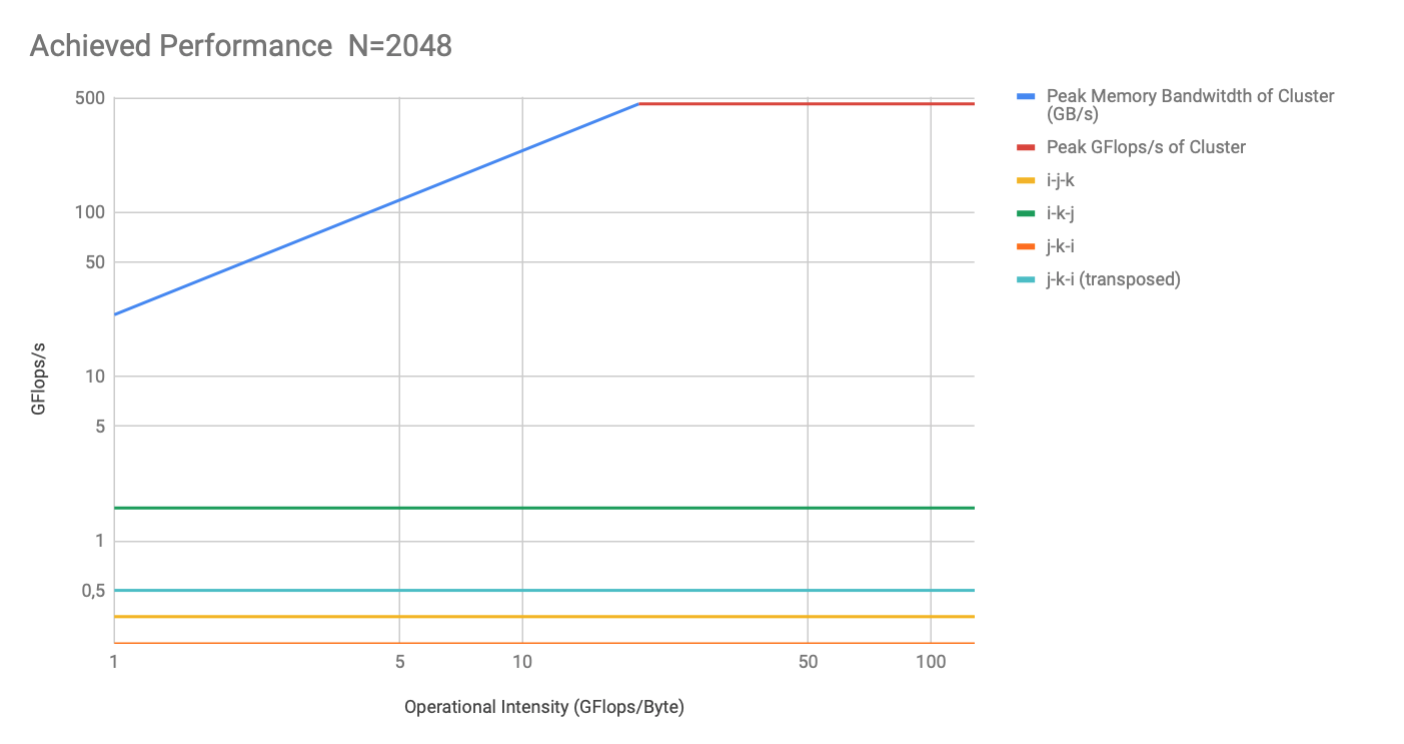
\includegraphics[width=15cm]{Pictures/roofline_ap_2048.png}
    \caption{Achieved Performance for N=2048}
    \label{fig:roofline_ap_2048}
\end{figure}

\section{Miss rate on memory reads}
\label{miss_rate}
\subsection{L1}
\begin{equation}
\frac{L1\_LDM}{LD\_INS}
\end{equation}

\subsection{L2}
\begin{equation}
\frac{L2\_DCM-L2\_STM}{L1\_LDM}
\end{equation}

\subsection{L3}
\begin{equation}
\frac{L3\_TCM}{L2\_DCM}
\end{equation}

\section{Block Optimization + Vectorization}

\begin{tabular}{|c|c|}
\hline
              & i-k-j \\
\hline
Matrix Order  & K-Best(K=3) and Tolerance (5\%) (us)  \\ 
\hline \hline
 52           & 31,00$\pm$1,55 \\
\hline
 128          & 458,33$\pm$22,92 \\
\hline
\end{tabular}

\section{Block Optimization + Vectorization + Multi core}
\begin{tabular}{|c|c|}
\hline
              & i-k-j \\
\hline
Matrix Order  & K-Best(K=3) and Tolerance (5\%) (us)  \\ 
\hline \hline
 2048         & 287100,33$\pm$14355,02 \\
\hline
\end{tabular}

\section{K20m}
\label{kepler_k20m}
\begin{tabular}{|c|c|c|}
\hline
              & \multicolumn{2}{|c|}{i-k-j} \\
\hline
Matrix Order  & K-Best(K=3) and Tolerance (5\%) (us) & data transfer times (us)  \\ 
\hline \hline
 2048         & 30583,00$\pm$1529,15 & 30563,00 \\
\hline
\end{tabular}

\section{KNL with Block Optimization + Vectorization + Multi core}

\begin{tabular}{|c|c|}
\hline
              & i-k-j \\
\hline
Matrix Order  & K-Best(K=3) and Tolerance (5\%) (us)  \\ 
\hline \hline
 2048         & 239057,33$\pm$11952,87 \\
\hline
\end{tabular}

\section{Baseline vs. Blocking+Vectorization}
\begin{figure}[H]
    \centering
    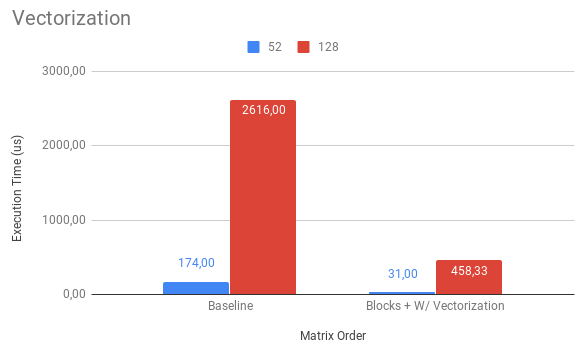
\includegraphics[width=15cm]{Pictures/exeTimeVec.png}
    \caption{Execution Time with 4 blocks size}
    \label{fig:exeTimeVec}
\end{figure}

\begin{figure}[H]
    \centering
    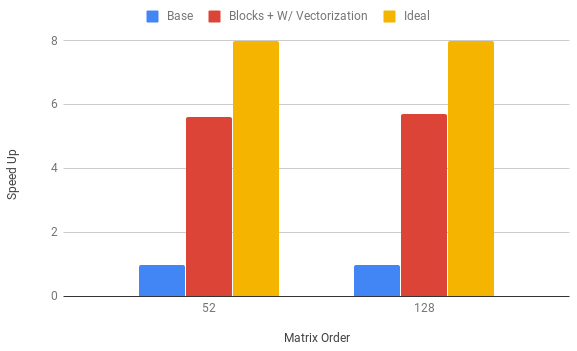
\includegraphics[width=15cm]{Pictures/speedUpVec.png}
    \caption{Speed Up}
    \label{fig:speedUpVec}
\end{figure}

\section{Baseline vs. Blocking+Vectorization+Multicore}
\begin{figure}[H]
    \centering
    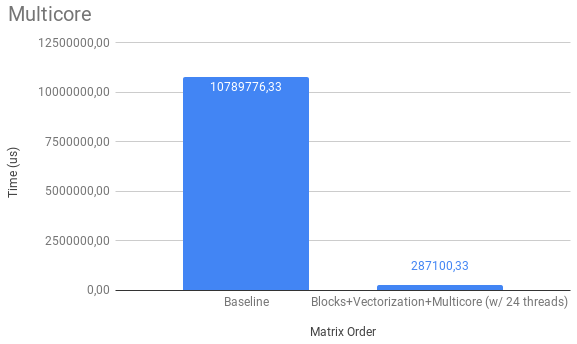
\includegraphics[width=15cm]{Pictures/exeTimeMulti.png}
    \caption{Execution Time with 4 blocks size}
    \label{fig:exeTimeMulti}
\end{figure}

\section{Baseline vs. Accelerators}
\begin{figure}[H]
    \centering
    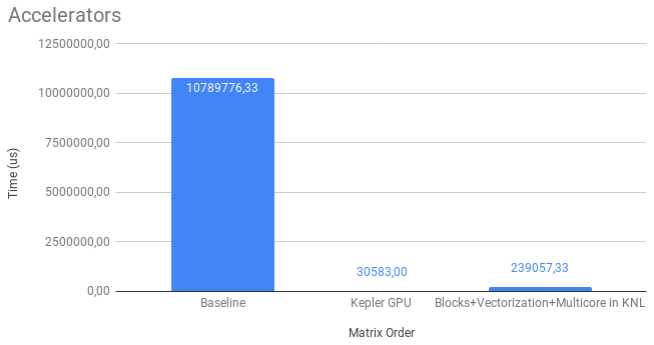
\includegraphics[width=15cm]{Pictures/exeTimeAcc.png}
    \caption{Execution Time with 4 blocks size (Only for KNL) for N=2048}
    \label{fig:exeTimeAcc}
\end{figure}

\begin{figure}[H]
    \centering
    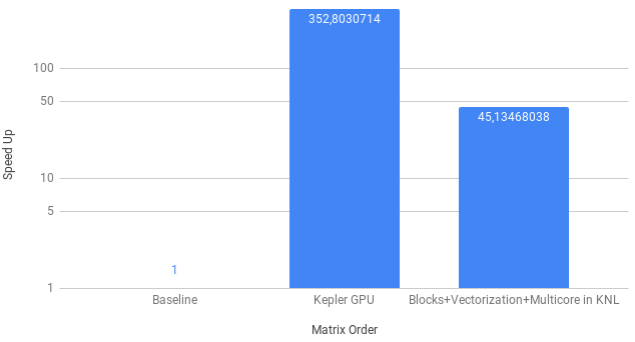
\includegraphics[width=15cm]{Pictures/speedUpAcc.png}
    \caption{Speed Up}
    \label{fig:speedUpAcc}
\end{figure}

\section{General Speed Up}
\begin{figure}[H]
    \centering
    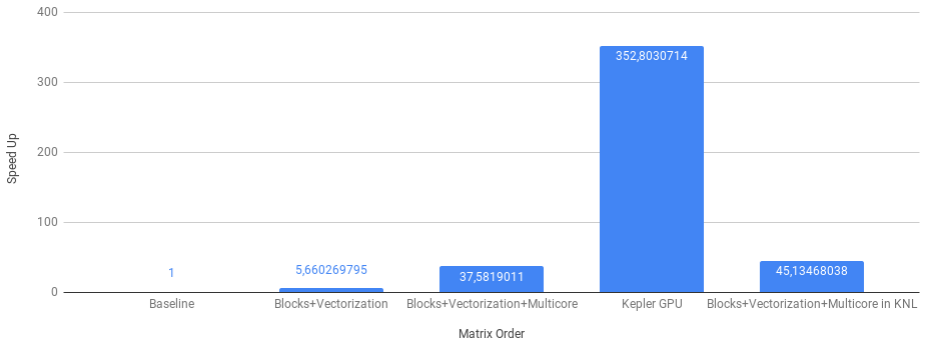
\includegraphics[width=15cm]{Pictures/generalSpeedUp.png}
    \caption{Speed Up}
    \label{fig:generalSpeedUp}
\end{figure}

\end{appendices}

\end{document}